\section{Математическая модель распростраанения эпидемий}
Succeptible Ill Resistant или SIR модель -- модель распространения эпидемий в изолированной популяции, описанная Кермаком В.О. и Мак Кендриком А.Г. в 1927 году. Данная модель не потеряла актуальности и в современных исследованиях.
Модель допускает три взаимосвязанных состояния при фиксированной популяции: 
\begin{figure}[H]
	\begin{center}
		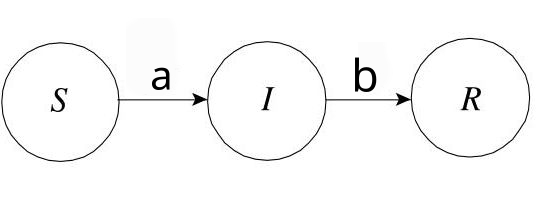
\includegraphics[width=0.7\linewidth]{ch11/SIR_model.jpg}
	\end{center}
	\caption{Графическая интерпретация взаимосвязей в модели SIR.}
\end{figure}
Так в данной модели однажды переболевшие имеют полный иммунитет.
\begin{equation}
	\left\lbrace 
	\begin{array}{lll}
		\frac{d(S+I+R)}{dt} &= 0,&\\
		\frac{dS(t)}{dt} &= -aS(t)I(t),& S(0)=S_0,\\
		\frac{dI(t)}{dt} &= aS(t)I(t)-bI(t),& I(0)=I_0,\\
		\frac{dR(t)}{dt} &= bI(t), R(0)=0,& S_0+I_0=N.
	\end{array}
	\right.
	\label{SIR_def}
\end{equation}
Заметим что последнее уравнение в \ref{SIR_def} избыточно. \\
Проведем анализ возможного поведения системы:
$\exists t, I(t)>I_0 \Rightarrow \dot{S}(t) \leqslant 0 \Rightarrow S(t) \leqslant S_0;$ $\dot{I} = I(t)(a(S(t) - b)$. Тогда если $S_0 < \frac{b}{a} \Rightarrow I(t) \leqslant I_0 \Rightarrow \text{эпидемии нет}$, но в случае $S_0 > \frac{b}{a}$ начнется эпидемия. Введем $\rho = \frac{b}{a}$.\\
\begin{equation*}
	\begin{array}{l}
	\frac{dS}{dI} = \frac{-aSI}{aSI-bI}=-\frac{aS}{aS-b}, I+S-\rho \ln{S}=I_0+S_0- \rho \ln{S_0} \leftarrow \text{Первый интеграл},\\
	\\
	\frac{dI}{dS} = -1 + \frac{\rho}{S}	
	\end{array}
\end{equation*}
При $S=\rho$ достигается максимум инфицированных и $\dot{I} = 0$ --- критическая точка. Вычислим максимальное число инфицированных: $I_{max} = \rho \ln{\rho} - \rho + I_0-\rho \ln{S_0} +S_0 =$ $= N-\rho +\rho \ln{\frac{\rho}{S_0}}$, $I = I_0 + S_0$ 
\begin{figure}[H]
	\begin{center}
		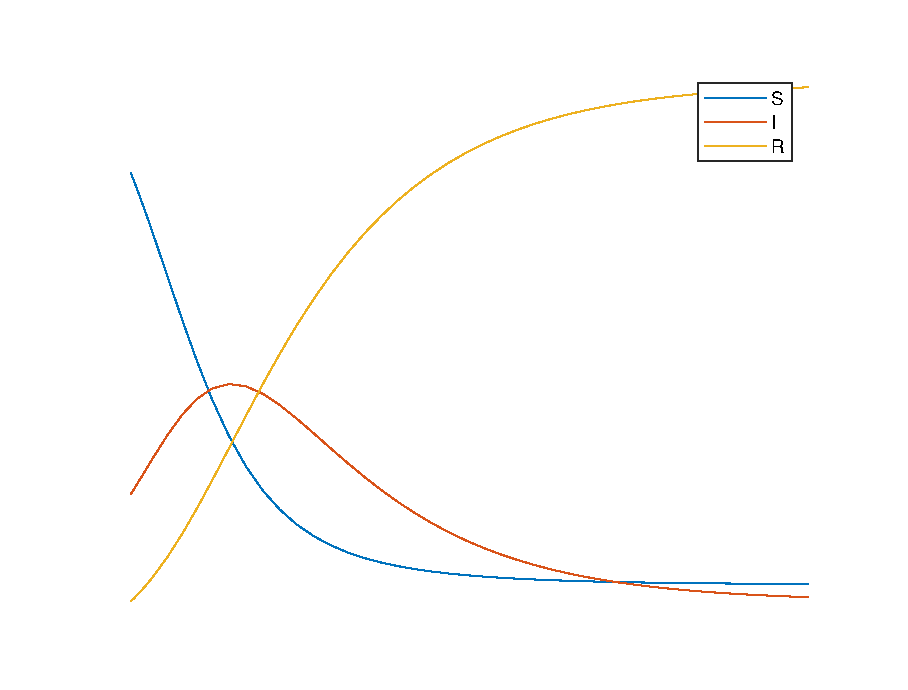
\includegraphics[width=0.7\linewidth]{ch11/SIR_graph.eps}
	\end{center}
	\caption{Типичное поведение системы SIR.}
\end{figure}

\section{Понятие средней приспособленности}
Рассмотрим некоторую популяцию, разбитую на субпопуляции $\left\lbrace N_{i}(t) \right\rbrace^n_{i=1}$, каждая из которых размножается в соответсвии с законом Мальтуса: $\frac{dN_{i}(t)}{dt}=r_{i}N_{i}(t)$. Перейдем от абсолютныхх численностей к относительным: 
\begin{equation*}
	p_{i}(t) = \frac{N_{i}(t)}{\sum_{k=1}^{n}N_{k}(t)}, \sum_{i=1}^{n}p_{i}(t)=1 \leftarrow \text{симплекс.}
\end{equation*}
\begin{figure}[H]
	\begin{center}
		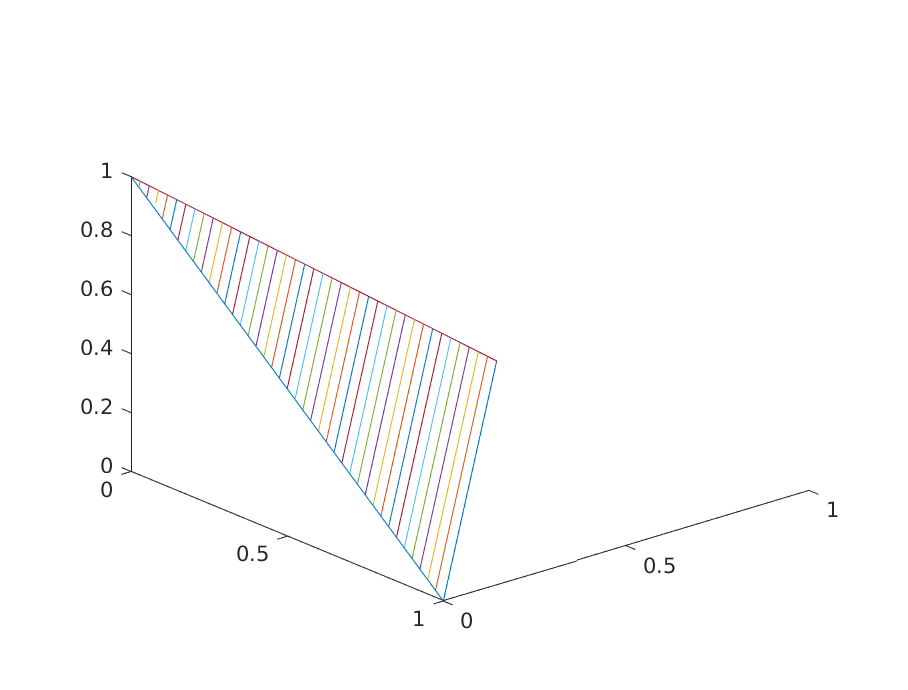
\includegraphics[width=0.57\linewidth]{ch11/simplex.eps}
	\end{center}
	\caption{Пример симплекса.}
\end{figure}
\begin{equation*}
\begin{array}{l}
	\dot{p}_{i}(t) = \displaystyle \frac{\dot{N}_{i}\sum_{k=1}^{n}N_{k} - N_{i}\sum_{k=1}^{n}\dot{N}_{k}}{(\sum_{k=1}^{n}N_{k})^2} =\\
	\\
	= \displaystyle\frac{r_{i}N_{i}\sum_{k=1}^{n}N_{k} - N_{i}\sum_{k=1}^{n}r_{k}N_{k}}{(\sum_{k=1}^{n}N_{k})^2} = r_{i}p_{i} - p_i\sum_{k=1}^{n}r_{k}p_{k}
\end{array}
\end{equation*}
Так мы получили уравнение второго порядка для введенной нами относительной величины, которая при этом в любой момент времени является симплексом. Здесь $r_i$ --- приспособленность $i$-го вида, а величину $f(t)=\sum_{k=1}^{n}r_{i}p_{i}$ принято назвывать средней приспособленностью или, как её называют в иностранной литературе, фитнессом системы. Получается что наиболее приспособленные виды выживают и плодятся, а менее приспособленные виды со временем исчезают, причем данная модель допускает появление новых видов со временем (их изначальная численность изначально была равна 0). Вычислим производную средней приспособленности:
\begin{equation*}
	\begin{array}{rl}
		f(t) &= \sum_{k=1}^{n}r_{k}p_{k}, \sum_{k=1}^{n}p_{k}(t) = 1;\\
		\dot{f}(t) &= \sum_{k=1}^{n}r_{k}\left(p_{k}r_{k} - p_{k}f(t)\right)=\\
		\sum_{k=1}^{n}r_{k}^{2}p_{k} - \sum_{k=1}^{n}r_{k}p_{k} \sum_{j=1}^{n}r_{j}p_{j} &= \sum_{k=1}^{n}r_{k}^{2}p_{k} - \left(\sum_{k=1}^{n}r_{k}p_{k}\right) > 0
 	\end{array}
\end{equation*}
Последняя часть равенства больше нуля и её можно рассматривать аналог дисперсии, при этом получаем, что средний фитнесс растет. Данный вывод был получен Рональдом Фишером и им он был сформулирован так: "Каждый организм ращвивается так, что средний фитнесс растет".
При этом имеет место быть эффект Независимой репликации: в итоге выживает только один вид $r^{*} = \max\limits_{1 \leqslant k \leqslant n}{\left\lbrace r_{k} \right\rbrace}$. Покажем это далее:
\begin{equation*}
	\dot{\left( \frac{p_{s}}{p_{i}} \right)} = \frac{\dot{p}_{s}p_{i} - \dot{p}_i p_{s}}{p_{i}^{2}} = \frac{p_{i}p_{s} \left( r_{s} - \sum_{k=1}^{n} r_{k}p_{k} \right) - p_{i}p_{s} \left( r_{i} - \sum_{k=1}^{n} r_{k}p_{k} \right) }{p_{i}^{2}} = \frac{p_{i}p_{s}\left(r_{s} - r_{i}\right)}{p_{i}^{2}}=
\end{equation*}
\begin{equation*}
\begin{array}{lr}
	= \displaystyle \left(r_{s} - r_{i} \right) \frac{p_{s}}{p_{i}} &\displaystyle \Rightarrow \frac{p_{s}}{p_{i}} = c_{0}e^{\left(r_{s} - r_{i} \right) t}
	\end{array}
\end{equation*}
Тогда возможны два случая:
\begin{enumerate}
	\item \hfill $
		r_{s} - r_{i} < 0 \Rightarrow \frac{p_{s}}{p_{i}} \underset{t\rightarrow \infty}{\longrightarrow} 0 \Rightarrow r_{i_0}=r^{*}$ \hfill \null
	\item \hfill $
		r_{s} - r_{i} > 0 \Rightarrow \frac{p_{s}}{p_{i}} \underset{t\rightarrow \infty}{\longrightarrow} \infty \Rightarrow \frac{p_{i_0}}{i} = c_{0}e^{\left(r^{*} - r_{i}\right)t}\underset{i \neq i_{0}}{\longrightarrow} \infty $ \hfill \null
		Здесь также получаем, что $p_i \rightarrow 0$ и $p_{i_0}$ --- ограничено, а тогда вся популяция сходится к виду $i_0$ и $p_{i_0} \rightarrow 1$ 
\end{enumerate}
Системы Лотки-Вольтерры --- не репликаторные. Репликаторная система: $\sum p_{i} = 1$.\\
Рассмотрим системы Лотки-Вольтерры:
\begin{equation*}
	\left\lbrace 
		\begin{array}{lll}
			\dot{u}_{i} &= u_{i} \left(r_i - \left(Au\right)_i\right), &i = \overline{1,n}\\
			\left(Au\right)_i &= \sum_{j = 1}^{n} a_{ij}u_{j}(t), &\left(Au, u\right) \geqslant \gamma \parallel u \parallel ^{2}, \forall u \neq 0, u > 0.
		\end{array}
	\right.
\end{equation*}
Здесь $r_{i} ~$ приспособленность, $f(t) = \left(Au, u\right)$ --- fitness. В данной системе fitness не всегда возрастает $\Rightarrow$ нужно менять члены матрицы $A$ --- ландшафт приспособленности.
\begin{equation*}
	\begin{array}{ll}
		\overline{u_{i}} &= \lim\limits_{t\rightarrow \infty} \frac{1}{t} \int_{0}^{t} u_{i}(t)dt,\\
		F &= \lim\limits_{t \rightarrow \infty} \frac{1}{t} \int_{0}^{t} f(t)dt \text{ --- средний fitness}
	\end{array}
\end{equation*}
Ответом системы будут резистентные клоны. Проблемы решения: сложность интегралов и большое множество видов.
%Далее рассмотрим систему, описывающую пищевую цепочку:
%\begin{equation}
%\left\lbrace 
%	\begin{array}{lll}
%		\dot{u}_{1} &=  &r_1 u_{1} - a_{12}u_2 - a_{11}u_1\\
%		\dot{u}_{2} &= -&r_2 u_{2} + a_{21}u_1 - a_{22}u_1 - a_{23}u_3\\
%		\dot{u}_{3} &= -&r_3 u_{3} + a_{32}u_2 - a_{32}u_2 - a_{33}u_3\\
%	\end{array}
%\right.
%\end{equation}
%Здесь матрица $A$ примет вид:
%\begin{equation*}
%\left(
%	\begin{array}{ccc}
%		a_{11} &  a_{12} &   0 \\
%	   -a_{11} &  a_{22} & a_{23} \\
%	    0   & -a_{32} & a_{33} \\
%	\end{array}
%\right)
%\end{equation*}
%И $\left(Au, u\right) =  a_{11}u_1^2 + a_{22}u_2^2 + a_{33}u_3^2 + a_{12}u_1 u_2 - a_{21}u_1 u_2 + a_{23} u_2 u_3 - a_{32}u_2 u_3 = a_{11}u_1^2 + a_{22}u_2^2 + a_{33}u_3^2 + u_1 u_2\left(a_{12} - a_{21}\right) +  u_2 u_3 \left(a_{23} - a_{32} \right)$, $\left(Au\right)_i = r_i, i = \overline{1,n}$.


